\documentclass[a4paper]{article}                                     
\usepackage{url,xspace,epsfig,etoolbox}
\usepackage{natbib}
\usepackage{fullpage}
\usepackage[font=bf]{caption}
\usepackage{mdwlist}
\usepackage{graphicx}

% No page numbers
\pagestyle{empty}

% Use 'Arial' font
\usepackage{helvet}
\renewcommand{\familydefault}{\sfdefault}

% Allow point-size specification of font
\usepackage{fix-cm}

% Allow setting margins on the abstract
\usepackage{changepage}

\newcommand{\projecttitle}{The Culture-Narration Genre: Defining the genre and identifying its potential for educational games}

% Prevent indentation of new paragraphs
\setlength{\parindent}{0pt}

% Put space after each paragraph. Note that this matches section titles too,
% and the workaround is below.
\setlength{\parskip}{\baselineskip}

% Allow easy overriding of section and subsection commands
\usepackage{titlesec}
\titleformat{\section}{\bfseries\fontsize{12}{14.4}\selectfont}{}{0em}{}
\titleformat{\subsection}{\bfseries\fontsize{11}{13.2}\selectfont}{}{0em}{}

% No blank line after section titles.
\titlespacing{\section}{0pt}{0pt}{-\baselineskip}
\titlespacing{\subsection}{0pt}{0pt}{-\baselineskip}

% No blank spaces between references
\setlength{\bibsep}{0pt}

% Hanging indent of 0.5 inches in references
\setlength{\bibhang}{0.5in}

% Keep all the screenshot figures the same width
\newcommand{\screenshotwidth}{2.5in}

% Is this blind or not?
\newtoggle{blind}
\toggletrue{blind}

\begin{document}

% Title is bold, centered, 14pt.
% Standard baseline skip is 1.2*fontsize, or 16.8 here.
\begin{center}
\fontsize{14}{16.8}\selectfont
\bf \projecttitle
\end{center}

% Gleaning author placement information from the existing proceedings.
\vspace{-0.25in}
\begin{center}
\iftoggle{blind}{
 % Nothing here: skip authors for blind review
}{
Paul Gestwicki, others, Ball State University\\
pvgestwicki@bsu.edu\\
}
\end{center}

\newcommand{\totan}{\textit{TotAN}}
\newcommand{\smersh}{\textit{SMERSH}}

% Abstract: 150 words or less, extra 0.5in left and right margin.
% Note that all text is justified.
%
\begin{adjustwidth}{0.5in}{0.5in}
  \textbf{Abstract:} \textit{Culture-narration games} are a promising
  genre for transformative games. This genre can be defined formal and
  dramatic characteristics, and we identify tabletop games that belong
  to the genre.  Adding technological components to the game affords
  new interaction modes as well as convenient digital distribution. We
  describe our team's pilot project at creating a technology-enhanced
  culture-narration game to improve cultural empathy among players aged
  10--14.  This pilot project highlights several complications with
  this genre, including thematic, technical, and production
  challenges.  However, the pilot project justifies continued
  experimentation, development, and formal assessment within the
  genre.
\end{adjustwidth}

\section{Introduction}

\textit{Tales of the Arabian Nights}~\citep{Goldberg2009} is a 
tabletop board game based on the eponymous folk tale.
It was originally published in 1985~\citep{Goldberg1985} but is more commonly
known for its 2009 re-release. 
It is popular within the designer board game hobby with a board game
rank of 239 (thematic rank 75) on Board Game Geek as of this writing,
and Shut Up \& Sit Down rank it as the ninth best game of all 
time~\citep{ShutUp2015}.
In this game, players control a character within a mythical Arabian
setting, and players explore the known world to accumulate Story and
Destiny points. The winner is the one who is able to meet their 
Story and Destiny point goal while having a successful encounter
in Baghdad---the City of Peace.

An intriguing property of \textit{Tales of the Arabian Nights}~(hereafter, \textit{TotAN}) is that it eschews the conventional wisdom for game design,
that player immersion is related to agency.
When a player has an encounter in \totan, they are told the name of the
encounter---such as angry merchant,  powerful prince, or
elephant's graveyard---and based only on this information,
they must choose a reaction from one of the given tables; for example, 
table~$A$ contains options to grovel, aid, rob, avoid, converse,
attack, court, abduct, or honor.
Another player then reads a corresponding entry from 
the \textit{Book of Tales}, which is a~300-page
tome containing~2600 numbered entries.
Most entries provide introductory text followed by paragraphs
tagged with skills that the active player may choose to use---without
knowing the consequences. The reader then narrates the conclusion of the
encounter and informs the player of their rewards, often in terms of
Story or Destiny points, gaining new skills, finding treasures, or
gaining status cards that modify players' options in future encounters.
To summarize, the player chooses a location on the map, but they do not 
choose what is encountered; they choose a reaction to the encounter name
without knowing how it will be interpreted in the story;
if they have the corresponding skill, they may choose to use it but
without knowing whether it will help or hinder them.
\totan{} is not a game of skill, where the player with the best tactics
wins the game: it is somewhat arbitrary and imbalanced, but from its
design emerges a fanciful gameplay experience. It is not played to win
but rather to enjoy the emerging story with friends.

This property of \totan{} reflects several characteristics
of its source material---a book that ``changed the world on a scale
unrivalled by any other literary text''~\citep[p.1]{Makdisi2008}.
Our team focused on the translation by \citep{Neil1994}, a youth-friendly
version recommended in the \totan{} rulebook.
Like the original stories, \totan{} is a collection of shorter stories
that are sometimes linked together and sometimes not.
The characters in the folk tales are often victims of fate with
very little agency over their own encounters. The games rules follow
cultural norms expressed in the folk tales:
you cannot win while sex-changed or on pilgrimage, and both marriage
and children are great blessings---unless you have an ugly baby,
which is shameful.
Baghdad is the most important city in the world, where your adventure starts
and ends.
Furthermore, many stories in \totan{} come directly from the tales,
such as the Sindbad's escape from the valley of diamonds or Aladdin's
being trapped in a magic cave. 

Playing \totan{}  inspired members of our team to read translations
of the original tales, which made us recognize the cleverness of the design
and its elegant dovetailing with the source material.
Furthermore, in reading the texts, we recognized that we had already
learned elements of the stories and the culture through playing the game,
although not always consciously or explicitly.
This inspired the following analysis, in which we tease apart the
various elements of \totan{}, considering them from both game design
and learning design points of view, and then share the results of a pilot
project to create a technology-enhanced game within the same genre.

The role and meaning of narrative in games is a perennial topic
of discussion among game design theorists.
We hope to position this work not as one of ludology or narratology,
but more pragmatically as part of a systematic investigation of how
systems and stories interact to produce learning outcomes.

\section{Defining the genre of culture-narration games}

We propose that \totan{} is one of very few games comprising a genre
of \textit{culture-narration games}, and we define this genre as having
the following characteristics.

\begin{enumerate}
\item \textit{Take place in a believable, consistent setting.} 
 Although the world of \totan{} may be unfamiliar to the player,
 everything in it is representative of the world described in the original
 folk tale---complete with the contradictions that add depth and nuance.

\item \textit{Use narrative as a primary feedback mechanism.} 
 In \totan{}, the player's reaction and skill choice yields two forms
 of feedback: the narrative description followed by the changes to the
 game state. The narrative is primary, both chronologically and aesthetically.
 Note that we follow \citet{Koster2012} in treating narrative as a 
 feedback mechanism, not a game mechanism.


\item \textit{Have measurable goals.} There is a winning condition as part
 of the social contract of play, following colloquially-accepted 
 standards for board games. The ``game'' is not simply constrained
 cooperative storytelling or a role-playing experience without formal end
 conditions.

\item \textit{Incorporate endogenously meaningful ambiguous decisions.}
 Following \citet{Burgun2012}, the decisions that one makes in the game
 are meaningful even though they are made without complete knowledge
 of the game state. For example, a player makes 
 the choice of reaction in \totan{} in hopes that it leads toward skills
 that they have, such as choosing ``Fight'' while in possession of the
 ``Weapon Use'' skill, even though one does not know whether or not
 this skill will have relevance in the resulting entry from the
 \textit{Book of Tales}.

\item \textit{Reward players for decision-making that reflects
    cultural understanding.}  The knowledge that a player brings to
  bear on decisions is not just knowledge of in-game systems.  If one
  chooses to Fight an Angry Ifrit in \totan{} without the Weapon Use
  skill, it is probably not going to end well. This prediction is not
  based on my having memorized the \textit{Book of Tales}, nor knowing how many
  hit dice an Ifrit has (as in \textit{Dungeons \& Dragons} powergaming).
  Rather, this prediction draws upon a cultural understanding of anger,
  spirits, violence, and likely much more.
  However, the game does this without establishing
  ``right'' and ``wrong'' (``moral/immoral'',
  ``light side/dark side'', ``paragon/renegade'') choices.  There
  remain unexpected twists: perhaps fighting the Angry Ifrit without
  combat skills makes him respect you and grant a boon.  \totan{},
  after all, is a game that allows the player to choose to ``drink'' a
  violent storm or ``enter'' a mysterious artifact.  While the world
  remains consistent, it also embraces the potential for surprising
  results.

\end{enumerate}

Two formal elements from \totan{} are intentionally not included in the
genre definition above. Perhaps the most clear omission is players' reading
each others' stories. While we agree that this is a critical element of 
\totan{}---and that it dovetails performatively 
and practomimetically~\citep{Travis2011} with Scheherazade's
performances in the source material---it is not clear that this is
characteristic to the genre.  Anecdotal evidence shows that
players with low reading skills can ruin the play experience for other
players, while those players could have read their own stories, aloud or not.
Similarly, \totan{} permits a single-player experience which, while
having a different aesthetic, still seems to produce the same general outcomes
we described above.

The other formal element omitted from the genre definition is the use of an
explicit map. The map is an important tangible aspect of \totan{}, 
in particular with its representation of Baghdad as the largest, most
important city in the world. However, we also note that virtual spaces
can be represented without such an explicit map, such as in the MUD family
of games or choose-your-own-adventure books, both of which
use discrete spaces without giving them visual manifestation.

Analyzing \textit{Agents of SMERSH}~\citep{Maxwell2012} establishes that
these characteristics form a genre and not merely selected elements from one
game.
\smersh{} is a cooperative game set in the Cold War, with players as 
covert agents trying to stop the enigmatic Dr.\ Lobo. 
Players move across the world collecting resources and battling henchmen,
facing encounters clearly inspired by \totan{}: flip a card to read an
encounter title, choose a reaction from a table, hear an introduction,
and then get different results based on skills. Unlike \totan{},
\smersh{} uses dice for story resolution, and supporting resource
management mechanisms introduce important strategic decisions.
Despite the use of dice for story resolution, the feedback is still
primarily narrative.

For contrast, consider \textit{Above and Below}~\citep{Laukat2015}, a
worker-management game about building a city both above and below the
surface.  \textit{Above and Below} is primarily about building an
economic engine that generates victory points faster than your
opponents within a fixed number of rounds. Exploring the underground
is one source of points, and this is done by determining a random
entry within its encounter book.  A player reads this entry aloud,
after which the player is presented with a decision of how to
react. However, the reaction titles are a thin wrapper around a
risk-and-reward balance: each has a number which is the number of
successes required on dice rolls, so players choose the highest number
they believe they can roll. Higher numbers always equate to better results,
and this roll is usually the end of the encounter: a successful player
is given an in-game reward with no other story or narrative.
Hence, although \textit{Above and Below} includes an encounter book
that players read to each other, it does not satisfy the characteristics
to be in the culture-narration game genre.

\section{Cultural Empathy}

We have discussed how \totan{} uses cultural understanding, not only on a
small scale as a way to reward players, but also as a key takeaway of
the game. In order for the game to reward players for their cultural
understanding, we have to present cultures in a way that they can, to
some extent, be understood. In other words, our game needs to foster a
sense of \textit{cultural empathy}, defining ``empathy'' as 
the ``state of mind in which someone shares the feelings or outlook of
another, sometimes prompted by imaginative exercises 'stepping into
someone's shoes'''~\citep[p.242]{Honderich2005}
Therefore, cultural
empathy, loosely formed, is having empathy for others who are from
different cultures, which allows for better understanding of that
culture.

This goal of cultural empathy differs from a goal of \textit{cultural
literacy} which prepares individuals to participate in another culture
based on the information of the culture that they have been 
given~\citep[p.165]{Hirsch1983}. Being culturally literate is having the
ability to be able to participate in another culture that you are
``dropped into,'' similar to how being literate is having the ability to
understand or write a given work of text.  \totan{} focuses on a certain
level of literacy of the given culture. Players are rewarded for their
cultural understanding and their ability to ``perform'' in the given
culture because of the information they have. This is demonstrated in
the example above, understanding the cultural views of marriage and
sex-change have an important role in game play. However, cultural
empathy makes the main point the understanding, not the
performance. \totan{} relies on an understanding of cultural values as
opposed to just focusing on some of their values consequential
norms. Therefore, though \totan{} expects some sense of cultural
literacy, it focuses more on cultural empathy. When a player walks
away from the game they would not have gained the ability to
participate in either a Middle Eastern or South Asian culture;
however, they will have gained an understanding of that culture. 
%This
%is why our emphasis in creating the game has relied more on cultural
%empathy than cultural literacy. We focus more on a mindset of a
%culture, than about facts about the culture. 
In the context of the
game, cultural empathy is a means to the end of cultural
literacy. However, outside of the game, focusing on cultural literacy
within a semi-fictional world works as the means for cultivating
cultural empathy, particularly world culture empathy.

\section{Context}

Investigating the potential for culture-narration games to teach
cultural empathy brought our team into a partnership with
\textit{[a local library branch hidden for blind review]}. This branch
serves primarily patrons from low socio-economic status, although
its special technology education programs also draw homeschoolers from
around the region.
The youth patrons of the library tend to be 4rd--6th grade 
``latchkey kids'' who 
see the library as a place to visit with friends, to participate in programs,
and to access technology.

Conversations with program coordinators about culture-narration games
revealed that despite other differences, the youth patrons shared
a fascination with monsters, horror, and the macabre. 
This is in part because of cultural taboo: the youth will brag about
being able to see a PG-13-rated movie or play an M-rated game,
for example, and several kids worked together to produce an original
short movie based on battles between movie monsters.

The fascination exhibited by the youth patrons reflects various theses
of Cohen's monster theory~\citep{Cohen1996}. 
We see in their behavior that ``the same creatures who terrify and
interdict can evoke potent escapist fantasies''~(p.16).
Recognizing the youth patrons' attraction to this theme,
Cohen's theory establishing monsters as reflections of culture,
and the narrative potential of monsters,
our team decided to engage in a design experiment to validate our
hypotheses about culture-narration games,
in collaboration with \textit{the library branch}.


\section{Design Experiment}

A team of eleven undergraduate students, working with a faculty mentor,
undertook a design experiment and pilot study to explore a monster-themed
culture-narration game;
our approach draws upon constructionist~\citep{Papert2001}
traditions, engaging in the design experiment with a multifaceted approach,
building prototypes as a way to understand them.
The students' majors include Computer Science, English
(Creative Writing), Philosophy, Telecommunications (Audio Production),
and Art (Animation).
Each student earned three credit hours for the experience during a fifteen-week
semester,
working together in a studio space for two hours each Monday, Wednesday,
and Friday.
% In future version, cite the TOCE paper
The team collectively agreed upon three primary goals for the design
experiment in the cultural-narration genre:
to use narrative as the primary form of player feedback;
to teach cultural empathy;
and to use technology to address complications of analog implementations.

Given these goals, the team proceeded with an incremental and
iterative approach to game design and development.
The team used a design log to record design decisions~\citep{Cook2011},
and each iteration
produced an executable release in accordance with best practices of
agile software development~\citep[see, for example,][]{Cockburn2006,Keith2010}. 
Figures~\ref{fig:screenshots} and~\ref{fig:paper-prototype} demonstrate
design artifacts from the design and development process.
Each iteration was tested at
\textit{[the library branch]}, providing valuable feedback to the
team.  Each iteration concluded with a retrospective
meeting~\citep{Kerth2001}, which provided an opportunity for the
team's reflective practice~\citep{Schon1984}.
The results of these retrospectives included large and small changes
to the team's methodology, including a transition from
story mapping~\citep{Patton2014} to Scrum~\citep{Schwaber2013}.
In addition to paper prototypes, the team 
developed prototypes using JavaFX, PlayN, and Polymer, 
all of which allow for HTML5 Web deployment.
Game images and stories were inspired by the team's research on monsters
from world cultures, which included both research sources
(such as \citet{Cohen1996}) and children's books (especially
\citet{Steer2008} and \citet{Stowell2013}).
The team also consulted with local university experts on
games, monsters, world cultures, and literacy.


\newcommand{\figwidth}{2.5in}
\begin{figure}
\centering
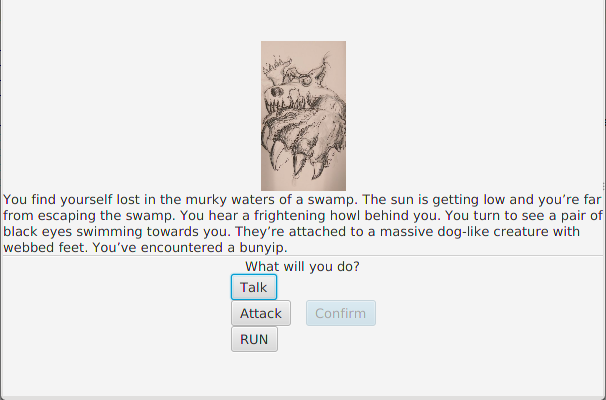
\includegraphics[width=\figwidth]{iteration-1}
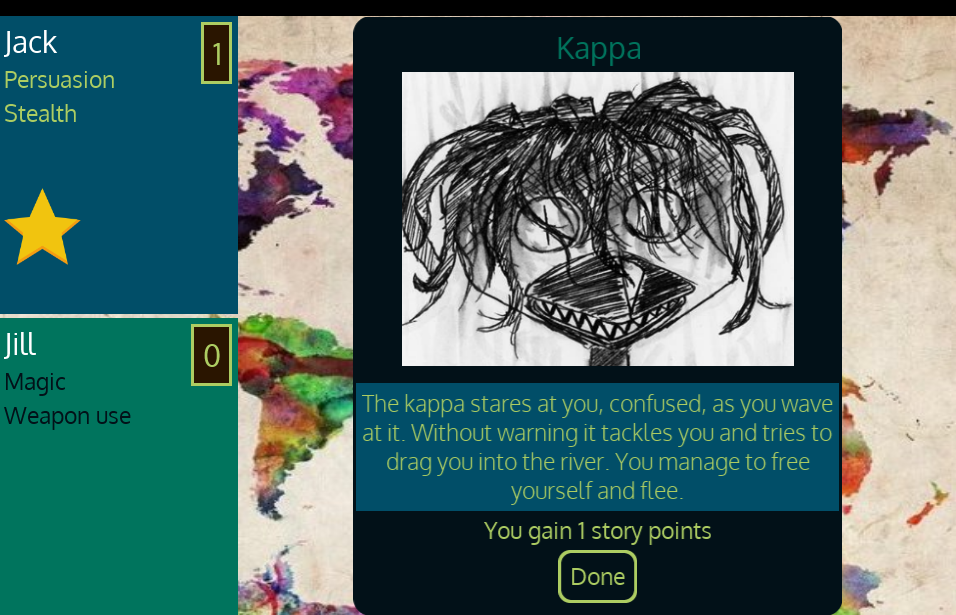
\includegraphics[width=\figwidth]{kappa-encounter}
\caption{Screenshots from Iteration 1 (left) and 2 (right)}
\label{fig:screenshots}
\end{figure}

\begin{figure}
\centering
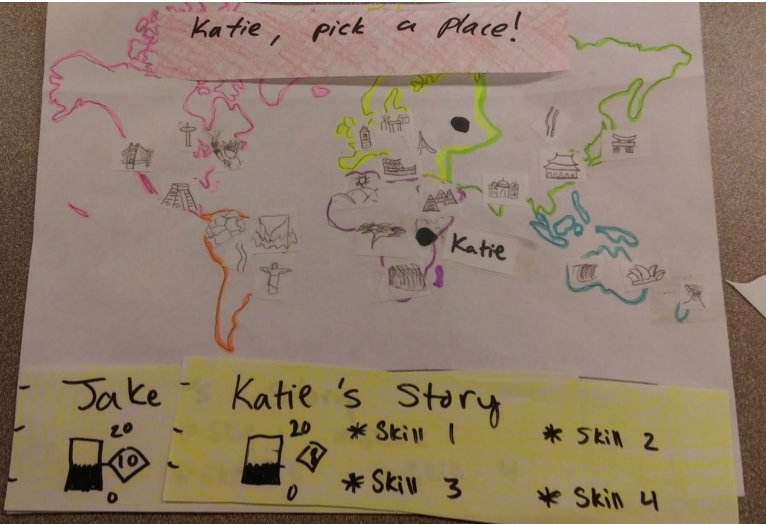
\includegraphics[width=\figwidth]{paper-prototype}
\caption{Paper prototype from Iteration 3}
\label{fig:paper-prototype}
\end{figure}


\section{Pilot Study}

\textit{In which we describe what playtesting has revealed to us}

\section{Conclusions and Future Work}

Based on our design experiments, pilot study, and understanding of the
literature, we believe there is a significant potential for
culture-narration games as learning tools, particularly for
cultural empathy.
However, as with any educational intervention, these games do not
come without complications.

Physical games such as \totan{} and \smersh{} are expensive to produce
and, for many, intimidating to encounter. \totan{}'s 19-page
instruction booklet may not faze a board game enthusiast, but we have
observed that others are intimidated by the large rulebook, heavy box,
and many components included in the game. Combined with the duration
of play and complexity of rules, such games seem inappropriate for use
in almost all formal educational settings such as conventional
schools.  However, we have found that the combination of technology
enhancement, grade-level writing, and shorter duration circumvents
these problems.  Digital implementations all but eliminate
distribution costs, and with clever game design, children can play the
game in the relatively chaotic environment of an informal after-school
program. With curriculum aides and improved scaffolding, such as
post-game debriefing, we are certain the game could be easily
integrated into school environments, particularly those with
ready access to computers.

The role of text within the game is worthy of particular attention.
The textual expression of narrative requires that players already possess
literacy skills: players who struggle with vocabulary or decoding words
are easily frustrated by such games. There is an opportunity
here as well, to differentiate text based on player reading level
or provide embedded reading aids; however, this also transforms
the outcome of the game from cultural empathy to reading literacy.
Player oration---having players read aloud to each
other---additionally requires oratory skills. We observed engagement
being enhanced when the reader employs theatrical talents as well.
The precise role of oratory skill, self-confidence, and the social
contract of gameplay (the ``magic circle'') is an area for future work.


\section{Acknowledgments}
\textit{The team, organizational, and community partner
  acknowledgments are hidden for blind review.}

\bibliographystyle{apalike}
\bibliography{references}

\end{document} 